\documentclass[11pt]{beamer}
\usetheme{Warsaw}
\usepackage[utf8]{inputenc}
\usepackage[spanish]{babel}
\usepackage{amsmath}
\usepackage{amsfonts}
\usepackage{amssymb}
\usepackage{graphicx}
\author{N.Pérez-Medina}
\title{Capítulo 3 - Métodos de espacio de fases.}
\setbeamercovered{transparent} 
\setbeamertemplate{navigation symbols}{} 
\logo{
\includegraphics[scale=0.04]{logo_fing_uach_bn.png} } 
\institute{\textbf{FING - UACH}
	\\
	\begin{small}
	\textit{Resumen del libro 'Análisis de series de tiempo no lineales' de Kantz y Schreiber}\\
	\end{small}
	
	\bigskip
	
	\begin{small}
	\textbf{Catedrático:} Dr. José Luis Herrera Aguilar
	\end{small}		
	} 
\date{\today} 
\subject{Series de tiempo} 


% Para tener un morado coqueto
\definecolor{lightPurple}{RGB}{186, 146, 209} % Morado claro
\definecolor{darkPurple}{RGB}{98, 54, 150}    % Morado oscuro
\setbeamercolor{structure}{fg=darkPurple} % Color principal para estructuras
\setbeamercolor{frametitle}{bg=darkPurple, fg=white} % Título del marco
\setbeamercolor{block title}{bg=darkPurple, fg=white} % Título de bloques
\setbeamercolor{block body}{bg=lightPurple!30, fg=black} % Cuerpo de bloques

\begin{document}

\begin{frame}
	\maketitle
\end{frame}

\begin{frame}
	\tableofcontents
\end{frame}

\section{Determinismo: unicidad en el espacio de fases}
\begin{frame} 
\tableofcontents[currentsection] % Solo muestra la sección actual
\end{frame}

\begin{frame}{Espacio de fases}
	\begin{block}{En general}
		Una gran clase de sistemas puede describirse por:
		\begin{itemize}
			\item Un conjunto de \textit{\textbf{estados}}
			\item Algún tipo de reglas de transición 
		\end{itemize}		 
	\end{block}
\end{frame}

\begin{frame}{Espacio de fases}
	\begin{block}{En general}
		Una gran clase de sistemas puede describirse por:
		\begin{itemize}
			\item Un conjunto de \textbf{\textit{estados}}
			\item Algún tipo de reglas de transición 
		\end{itemize}		 
	\end{block}
	\begin{block}{Entonces}
		Podemos establecer un \textit{espacio vectorial} para el sistema, de modo que especificar un punto en este \textit{espacio} defina el \textbf{\textit{estado}} del sistema y viceversa
	\end{block}
\end{frame}

\begin{frame}{Espacio de fases}
	\begin{small}
	Nos restringiremos al caso en el que el \textbf{\textit{espacio de fases}} es un \textit{espacio vectorial} finito dimensional $\mathbb{R}^m$.
	Un estado está especificado por un vector $x\in \mathbb{R}^m$
	
	\begin{block}{Entonces}
		Tenemos dos maneras de describir la dinámica:
		\begin{enumerate}
			\item Si tomamos al tiempo como una variable discreta, una transfomación $m$-dimencional
			\begin{equation}
			\mathbf{x}_{n+1} = \mathbf{F}(\mathbf{x}_n), \quad n \in \mathbb{Z}
			\end{equation}
			
			\item Si tomamos al tiempo como una variable continua, un sistema explícito de $m$ ecuaciones diferenciales ordinarias de primer orden.
			\begin{equation}
			\frac{d}{dt}\mathbf{x}(t) = \mathbf{f}(\mathbf{x}(t)), \quad t \in \mathbb{R}.
			\end{equation}
		\end{enumerate}
	\end{block}
	\end{small}
\end{frame}

\begin{frame}{Espacio de fases}
	\begin{block}{De esta forma}
	Una secuencia de puntos $x_n$ o $x(t)$, resolviendo las ecuaciones anteriores, se denomina \textit{trayectoria del sistema dinámico}, con $x_0$ o $x(0)$, respectivamente, como la condición inicial.
	
	\end{block}
\end{frame}

\section{Reconstrucción con retardos}
\begin{frame} 
\tableofcontents[currentsection] % Solo muestra la sección actual
\end{frame}


\begin{frame}{Reconstrucción del espacio de fases}
	\begin{block}{En general}
		Lo que observamos en un experimento NO es un objeto en el espacio de fases, sino una secuencia de mediciones escalares. Por lo tanto, debemos convertir las \textit{observaciones} en \textit{vectores de estado}.
	\end{block}
\end{frame}

\begin{frame}{Reconstrucción del espacio de fases}
	\small
	\begin{block}{Enfoque más común}
		 La serie temporal es una secuencia de mediciones escalares de alguna cantidad que depende del estado actual del sistema, tomadas en múltiplos de un tiempo de muestreo fijo:
		\begin{equation}
			s_n = s(\mathbf{x}(n\Delta t)) + \eta_n .
		\end{equation}
		Es decir, observamos el sistema a través de alguna función de medición $s$ y realizamos observaciones solo hasta cierto punto de fluctuaciones aleatorias $\eta_n$ , \textit{el ruido de medición}.
	\end{block}	
\end{frame}

\begin{frame}{Reconstrucción del espacio de fases}
	\begin{block}{Reconstrucción por retardos}
		Una \textit{reconstrucción con retardos} en $m$ dimensiones se forma entonces mediante los vectores $\mathbf{s}_n$, dados por
		\begin{equation}
			\mathbf{s}_n = (s_{n-(m-1)\tau}, s_{n-(m-2)\tau}, \ldots, s_{n-\tau}, s_n) 
		\end{equation}
		La diferencia temporal en número de muestras $\tau$ (o en unidades de tiempo, $\tau \Delta_t$) entre componentes de los vectores de retardo se denomina \textit{lag} o \textit{tiempo de retardo.}
	\end{block}
\end{frame}

\section{Encontrar un buen embebido}
\begin{frame} 
\tableofcontents[currentsection] % Solo muestra la sección actual
\end{frame}

\begin{frame}{Sobre los \textit{Teoremas de incrustación}}
	\begin{block}{Lo más importante}
		Garantizan que, para datos ideales libres de ruido, existe una dimensión $m$ tal que los vectores $s_n$ son equivalentes a los vectores del espacio de fases.
	\end{block}

\end{frame}

\begin{frame}{Sobre $m$}
	\begin{block}{En general}
		\begin{itemize}
			\item Buscamos concoerlo de forma precisa porque queremos explotar el determinismo con un esfuerzo computacional mínimo.
			\item Si un embebido de dimensión $m$ proporciona una representación fiel del espacio de estados, cualquier reconstrucción en $m_0 > m$ también lo hará
			\item Tomar un valor demasiado grande para $m_0$ no sería útil y correría el riesgo de “confundir” al algoritmo.
		\end{itemize}
	\end{block}

\end{frame}

\subsection{Vecinos falsos}
\begin{frame}{Razonamiento central}
	Si asumimos que la dinámica en el espacio de fases está representada por un campo vectorial suave
	\begin{block}{Entonces:}
		Las dos trayectorias que emergen de dos \textit{estados vecinos}, después de un intervalo de tiempo corto hacia el futuro, aún deberían permanecer como \textit{vecinos cercanos}. 
	\end{block}
\end{frame}

\begin{frame}{Vecinos falsos más cercanos}
	\begin{block}{Idea básica}
		Buscar puntos en el conjunto de datos que son vecinos en el espacio de incrustación $m$, pero que no deberían ser vecinos, ya que su evolución temporal futura es demasiado diferente.
	\end{block}
	\begin{block}{Método}
		Para cada punto de la serie temporal: 
		\begin{enumerate}
			\item Tomamos su vecino más cercano en $m$ dimensiones
			\item Calculamos la razón de las distancias entre estos dos puntos en $m + 1$ dimensiones y en m dimensiones 
		\end{enumerate}		 
		Si esta razón es mayor que un umbral $r$, el vecino era falso.
	\end{block}	
	
	
\end{frame}

\begin{frame}{Estadística a computar}
	\begin{block}{}
		Ahora, cuando denotamos la desviación estándar de los datos por $\sigma$ y usamos la norma máxima, la estadística a computar es

\begin{equation}
X_{fnn}(r) = \frac{\sum_{n=1}^{N-m-1} \Theta \left( \frac{|s_{n}^{(m+1)} - s_{k(n)}^{(m+1)}|}{|s_{n}^{(m)} - s_{k(n)}^{(m)}|} - r \right) \Theta \left( \frac{\sigma}{r} - |s_{n}^{(m)} - s_{k(n)}^{(m)}| \right)}{\sum_{n=1}^{N-m-1} \Theta \left( \frac{\sigma}{r} - |s_{n}^{(m)} - s_{k(n)}^{(m)}| \right)}
\end{equation}

donde $s_{k(n)}^{(m)}$ es el vecino más cercano a $s_n$ en $m$ dimensiones, es decir, $k(n)$ es el índice del elemento $k$ de la serie temporal diferente de $n$ para el cual $|s_n - s_k| = \min$. 
	\end{block}
\end{frame}

\begin{frame}{Sobre las funciones escalón de (5)}
\begin{block}{La primer funciíon escalón del numerador}
	Es uno si el vecino más cercano es falso.
\end{block}
\begin{block}{La segunda función escalón del numerador}
	Suprime todos aquellos pares cuya distancia inicial ya era mayor que $\frac{\sigma}{r}$
\end{block}
\begin{block}{Nota}	
 Puede haber algunos vecinos falsos incluso cuando se trabaja en la dimensión de incrustación correcta.
\end{block}

\end{frame}

\subsection{El retardo temporal}
\begin{frame}{Sobre el tamaño de $\tau$}
	\begin{block}{Si $\tau$ es pequeño}
		\begin{itemize}
			\item Los elementos sucesivos de los vectores de retardo están fuertemente correlacionados. 
			\item Todos los vectores sn se agrupan entonces alrededor de la diagonal en $\mathbb{R}^m$
		\end{itemize}
	\end{block}
	\begin{block}{Si $\tau$ es muy grande}
		\begin{itemize}
			\item Los elementos sucesivos ya son casi independientes
			\item Los puntos llenan una gran nube en $\mathbb{R}^m$
		\end{itemize}
		
	\end{block}

\end{frame}

\section{Gráficas de recurrencia}
\begin{frame} 
\tableofcontents[currentsection] % Solo muestra la sección actual
\end{frame}

\begin{frame}{Idea central}
	\begin{block}{\textit{\textbf{Recurrencia}}}
		 El retorno de una trayectoria en el espacio de estados a una vecindad de un punto donde ya ha estado antes es lo que llamamos una \textit{repetición aproximada}. Cuando ocurre en una incrustación que representa un espacio de fases determinista entonces se llama \textit{\textbf{recurrencia}}
	\end{block}
	
	
\end{frame}

\begin{frame}{Construcción}
	\begin{block}{}
        Se define la matriz de recurrencia:
        \[
            M_{ij} = \Theta(\varepsilon - \| s_i - s_j \|),
        \]
        donde:
        \begin{itemize}
            \item $\Theta$ es la función escalón de Heaviside 
                  ($\Theta(x) = 1$ si $x \geq 0$, $0$ en caso contrario).
            \item $\varepsilon$ es el umbral de tolerancia.
            \item $\| s_i - s_j \|$ es la distancia entre los vectores en tiempos $i$ y $j$.
        \end{itemize}
    \end{block}
\end{frame}
    
\begin{frame}{Interpretación}
	\begin{block}{}
        \begin{itemize}
            \item $M_{ij} = 1$ si los estados son cercanos.
            \item $M_{ij} = 0$ si son lejanos.
            \item Al graficar $M_{ij}$ en un plano de índices, se obtiene la 
                  \textbf{gráfica de recurrencia}, con puntos negros (1) y blancos (0).
        \end{itemize}
    \end{block}
\end{frame}

\begin{frame}{¿Qué información nos da?}
	\begin{block}{}
		\begin{itemize}
			\item En un sistema determinista se espera que los puntos negros aparezcan típicamente como segmentos de línea cortos paralelos a la diagonal.
			\item Si además hay muchos puntos aislados, indica una fuerte componente de ruido en los datos, o una dimensión de embebido insuficiente
			\item Si hay principalmente puntos dispersos, el componente determinista está ausente o al menos es débil.
		\end{itemize}
	\end{block}
\end{frame}

\begin{frame}{Idea gráfica}
	\centering
	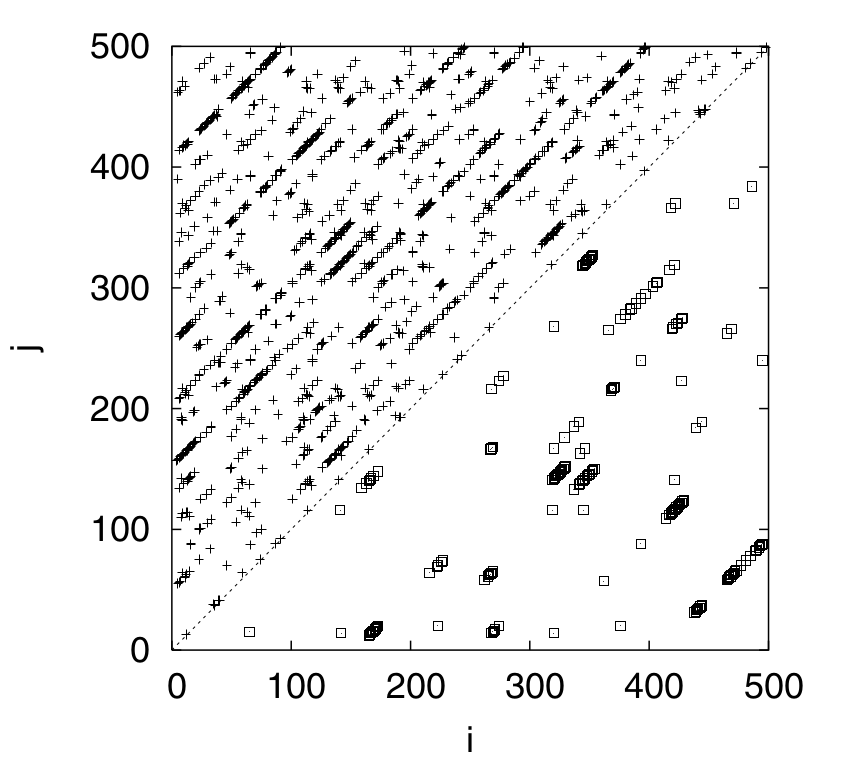
\includegraphics[scale=0.27]{grafica-recurrencia.png} 
\end{frame}

\section{Ejercicios}
\begin{frame} 
\tableofcontents[currentsection] % Solo muestra la sección actual
\end{frame}
\begin{frame}{Pasamos a los ejercicios}
	\begin{center}
		\Huge
		Gracias
	\end{center}
\end{frame}
\end{document}
\end{document}